% Hanrich Potgieter		
% Check 
subsubsection*{Integratability A}
We tested the Integratability of the following fucntions. These functions has been supplied by group A
\begin{itemize}
	\item Installing required Packages
	There is no way of installing the required packages.
	\item Dependancy Injection
	There is no dependacy injection.
	\item Unit tests
	There was no supplied unit test. Therefore we cannot test if the functions is working.
\end{itemize}
\subsubsection*{Integratability B}
The integratability of notification B is not adequite. There are numerbour challanges that are missing. There is no dependancy injection and all packages needs to be installed manually.
\begin{itemize}
	\item {File Structure} 
	Each function is placed in a seperate file. There is no common module to integrate that will allow access to all the capabilities of notifications.
	\item Installing required packages
	One cannot easily install the dependancys that is required by Notifications.
	\item Dependancy Injection
	There is no dependacy injection.
	\item
	Inappropriate Unit testing. Therefore we cannot test if the functions is working. There is a file called test.js that is an attempt at unit testing but no proper unit testing was applied. They should have used someting similar to Unit.js with mocha.
		~\ref{fig:IntegrationUnitTest}
		\begin{figure}[H]
			\centering
			\fbox{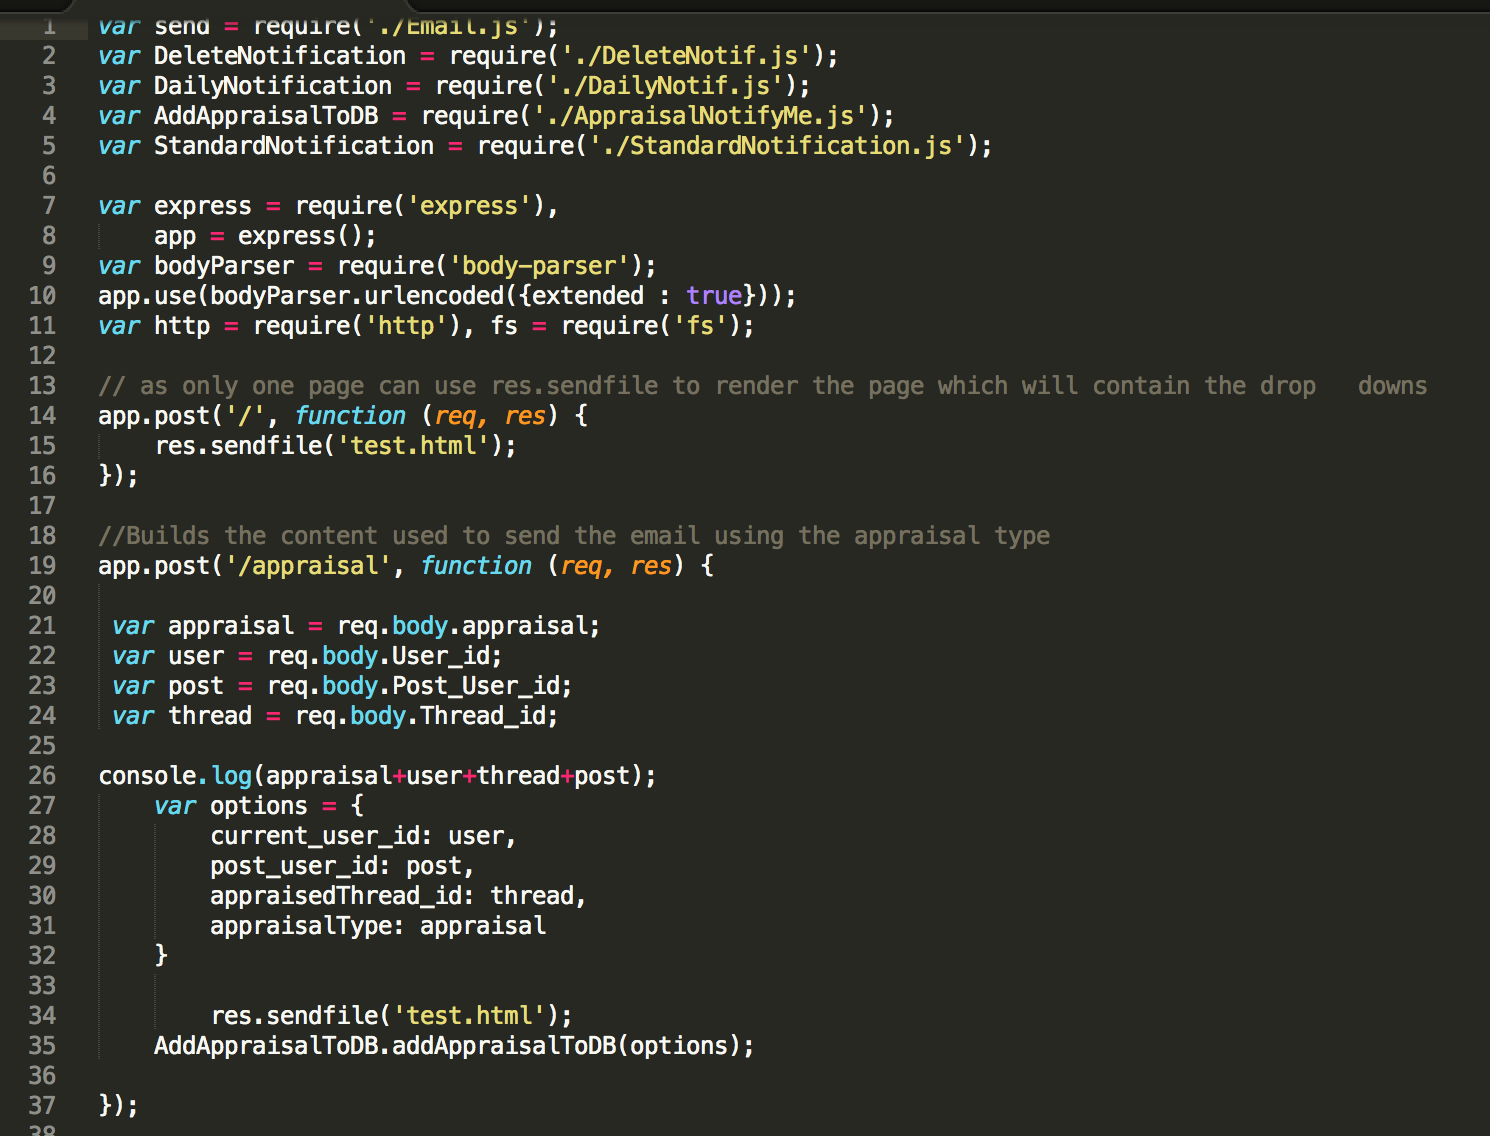
\includegraphics[width=1.0\textwidth]{IntegrationUnitTest}}
			\caption{Unit Tests}
			\label{fig:scope}
		\end{figure}
	\item database issues
	There is no way to access the specified database and this also contributes to the integratability. They sould supply a way to specifiy the database to be used.
		~\ref{fig:IntegrationDatabaseFail}
		\begin{figure}[H]
			\centering
			\fbox{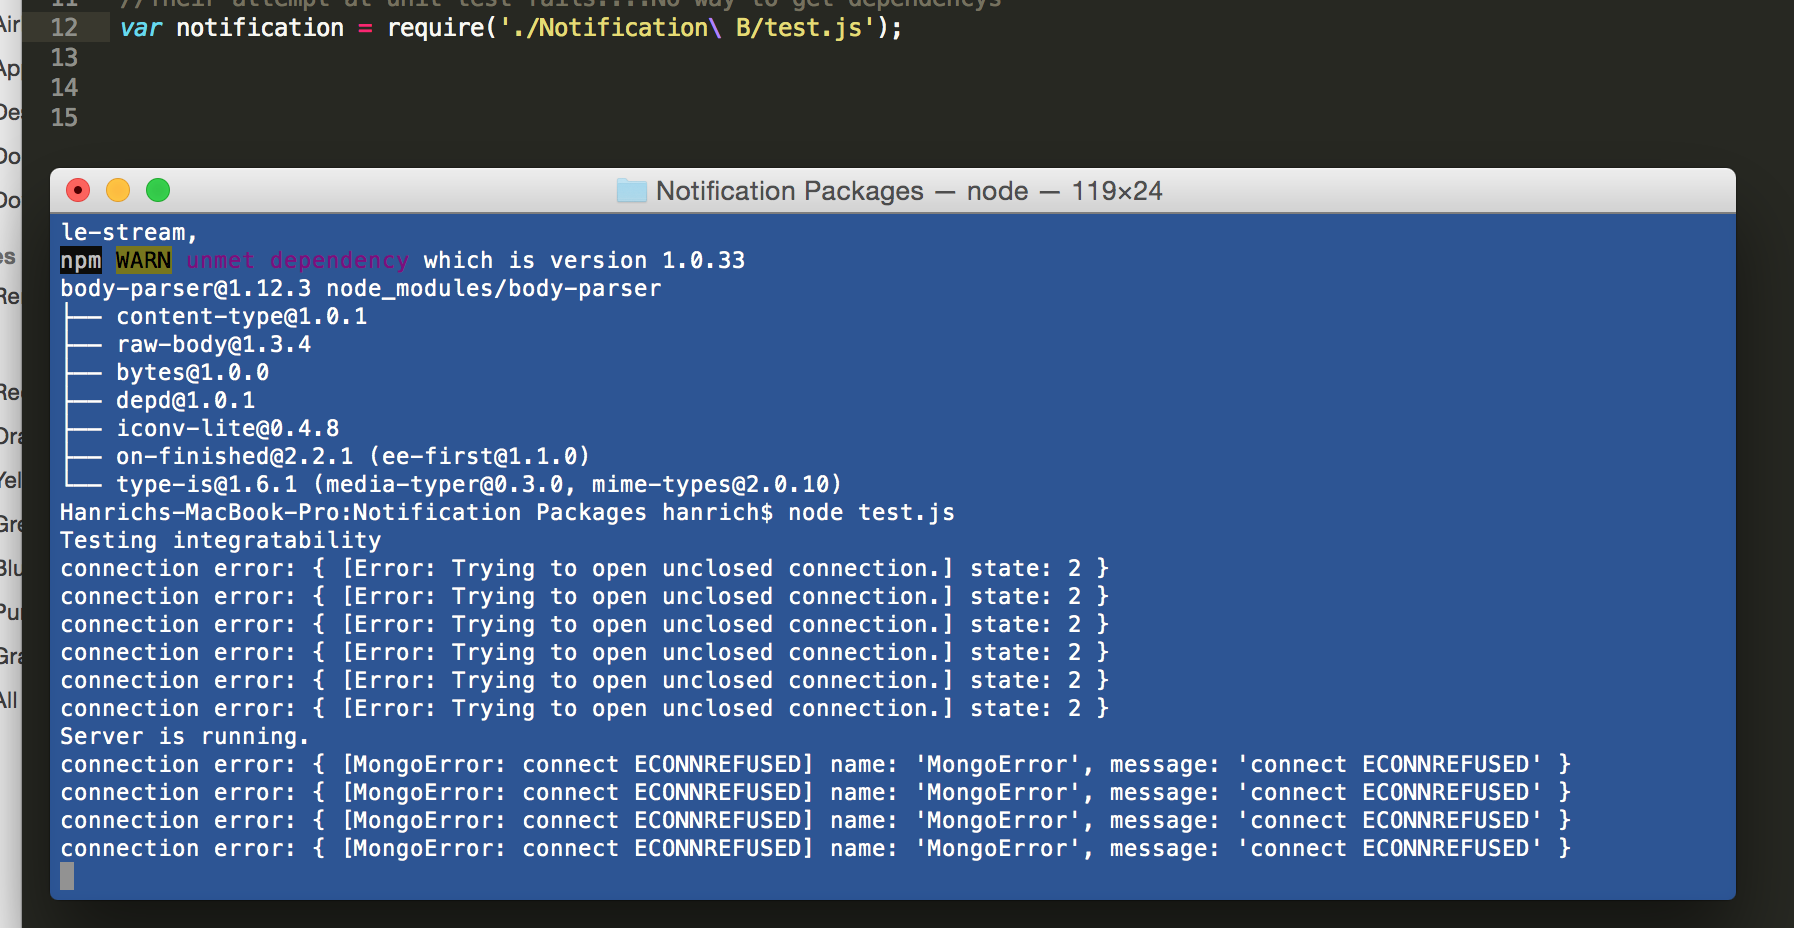
\includegraphics[width=1.0\textwidth]{IntegrationDatabaseFail}}
			\caption{Database connection issues}
			\label{fig:scope}
		\end{figure}
\end{itemize}
\subsubsection*{Remarks}
Notification B is not Integratable at alll. There is no provision for dependacny injection.